\section{Introduction}
\label{sec:introduction}

%{\color{blue} In this section we will contextualize video streaming technology and hierarchical caching problems, emphasizing the need of create a hierarchical topology to , and describe the content of each section of the paper.}

% Introduction of the Content and MEC service provider 
Over the years, Internet traffic has grown exponentially around the world, mainly due to multimedia content streaming, which currently represents 70\% of the whole traffic~\cite{cisco:forecast}. 
The Over-the-top~(OTT) provider can use the network edge to cache and transmit the video traffic with an uninterrupted streaming experience, as smooth as possible, to accommodate this growing video demand. This includes standard video services as well as innovative services such as real-time video streams, and future gaming platforms using cloud infrastructures~(e.g., AWS Wavelength and Google Stadia)~\cite{amzo:AWSEdge}.
This trend imposes new challenges in video provisioning to satisfy the Quality of Experience~(QoE) guarantees for a wide range of subscribers. As it was originally designed to consider the best-effort internet model for data transmission~\cite{gamaUCC2019, DBLP:CoRR:2021, ye:ITC17}.
%In order to provide the best user satisfaction, the advantages of high datarate and low latency in the edge network take into account today~\cite{gamaUCC2019, DBLP:CoRR:2021, ye:ITC17}. This trend imposes new challenges in providing videos with the best QoE, originally designed considering the best-effort internet model for data transmission.

When the content provider saturates available bandwidth or a particular set of service metrics across the network, the cloud server~(OTT provider) can reroute active connections to one or more edge caches to service the required demand. Such a model can be represented by a network organized hierarchically in multi-tiers to maintain a distributed, balanced traffic load~\cite{rosarioSENSORS2018}.
%When the content provider saturates the available bandwidth or a certain set of service metrics, the request may be routed to one or more edge caches. This model may be organized hierarchically in multi-tiers maintains a low traffic load~\cite{rosarioSENSORS2018}.

% Challenges
Using the edge of the network with cache and replica capabilities helps improve user satisfaction, but it can also bring negative impacts. When many users start to request video segments at the edge nodes, these surrogated nodes consider static users and just one edge node tiers. These nodes are not ready to deal with the constant changes in the number of users and switching between different Access Points~(AP) due to user mobility.
Several works of literature highlight edge/cloud computing to deal with the new video traffic demands, but there are neglected aspects related to dynamic load solutions. 

Figure~\ref{fig:multi-tier-network} depicts a multi-tier network architecture, which is composed of a heterogeneous set of devices and applications using distributed computing resources through multi-access communication technology. Below the cloud layer, the network edge is divided into three layers organized hierarchically. Core Network Regional Edge can manage coordination across the distributed infrastructure in this multi-tier ecosystem, for example, in a smart city, followed by the Access Network Edge, which supports a few dozen to maybe a few hundred local nodes at the middle layer of the edge computing infrastructure. The Edge gateways can be distributed on local edge nodes, where the node re-transmits video content employing wired or wireless communication.

\begin{figure}[htb!]
    \centering
    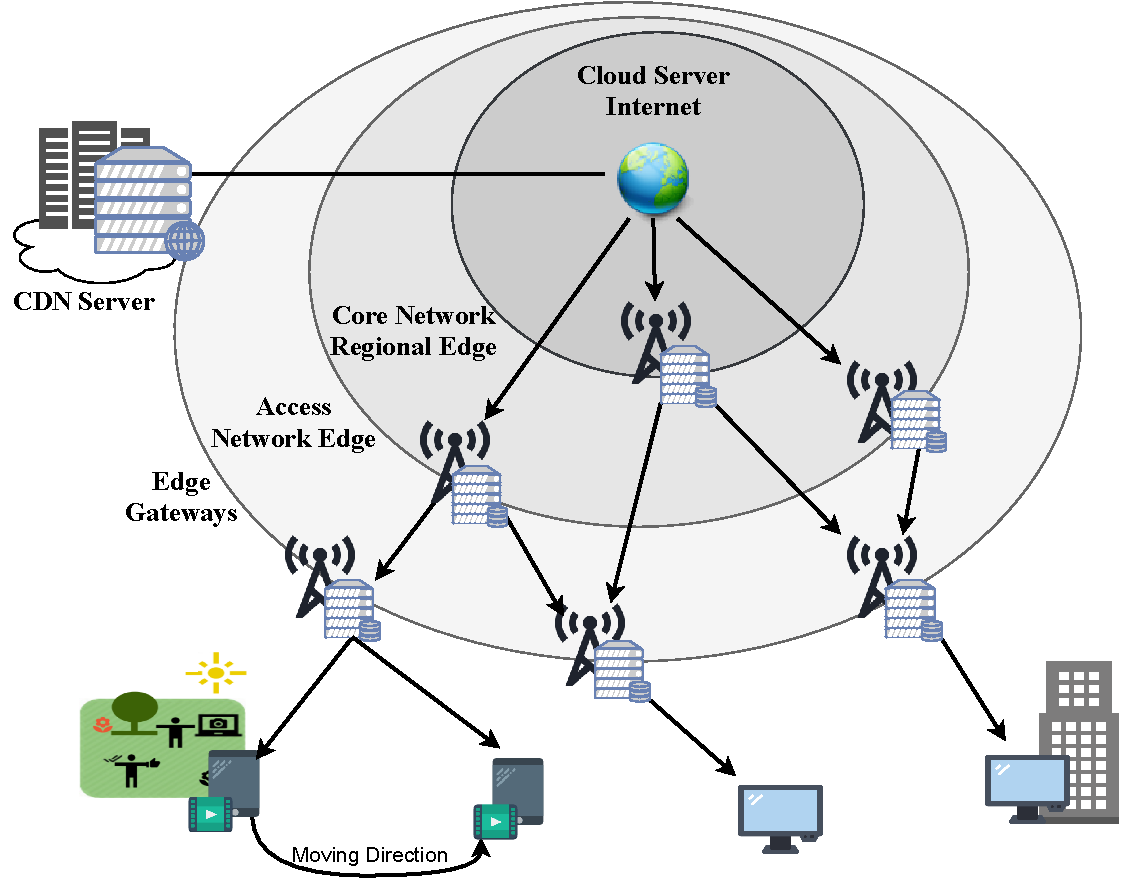
\includegraphics[width=\linewidth]{images/arch-video-content-2.pdf}
    \caption{A General Overview of the multi-tier network environment.}
    \label{fig:multi-tier-network}
\end{figure}

%
%Furthermore, the number of users connected in different APs changes accordingly to the surrogated edge nodes. For instance, a core network regional edge node provides video streaming to more users than an edge gateway. As shown in Fig.~\ref{fig:multi-tier-network}.
%
%Since the triggered video segments caching (replication) in an edge node.
%However, certain precautions when choosing the nodes for caching the video need to be taken into account. 

%Which it could result some issues. 

% Objective
Motivated by the characteristics mentioned above in multi-tier edge/cloud scenarios to improve users' satisfaction and accommodate the growing video traffic, this paper discusses the need for an orchestrator to provide video streaming content in dynamic scenarios.
Our goal is to provide designers and operators a performance analysis of a hierarchical edge network and its impacts on the users' QoE. In this paper, the models we present are evaluated by a series of simulations using a controlled environment, suggesting that dynamic resource allocation mechanisms are necessary to cope with video demands, such as when users are mobile.

% Organization paper
This paper is organized as follows.
Section~\ref{sec:related-work} presents the related work on the impact of edge/cloud networks on video streaming services.
A brief analysis of the proposed multi-tier edge/cloud network and a description of some opportunities of using such architectures are given in Section~\ref{sec:system-archi}.
Furthermore, Section~\ref{sec:results} shows the preliminary results on the impact of the network performance for video streaming services and motivates further research on the topic, and Section~\ref{sec:conclusion} concludes the paper.
